The handling of multiple actions for the same goal would bring us closer to what
\emph{auto} or \emph{tauto} do in Coq. We could have whole theories compiled in some sort
of database and let our tool figure out which of those lemmas to apply. Since the goal is
fixed, there should be one solution. A naive extension to our library could be made:

\Agda{RW}{by+-def}

However, a \F{List} of names is a bad data structure to use here. We need to search
every single action, where, we could rule out actions purely based on their structure.
Indeed, we are going to explore an alternative data structure to speed up search and get
instantiation for free, during lookup.

\begin{TODO}
  \item cite Tries, Edward Fredkin
\end{TODO}

This section starts with a summarized explanation of Tries and then follows with our
generalization of the same concept. The structure we arrive at is a type-indexed data structure,
in the sense of \cite{Hinze04}. Yet, our lookup and insertion methods have to be significantly different
since we have to handle variables, that can be arbitrarily instantiated.

\subsection{Tries}

There a few variations on of a Trie, suited for different applications. We will, however,
restrict ourselfes to the original definition, which is also the simplest. This small digression
has the purpose of introducing the underlying idea without too many technicalities.

\begin{wrapfigure}{r}{0.30\textwidth}
\begin{center}
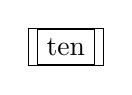
\begin{tikzpicture}[
  cnode/.style={rectangle , draw=black , fill=white},
  lbl/.style={circle , draw=none , fill=white , inner sep=0cm , font={\tiny \color{blue}}}
]
\tikzset{level 0+/.style={level distance=2cm}}
\Tree [.\node[cnode]{$\epsilon$};
        \edge node[pos=0.5 , lbl] {t};
        [.\node[cnode]{t};
           \edge node[pos=0.5 , lbl] {o};
           [.\node[cnode]{to};
             \edge[dashed] node[pos=0.5 , lbl] {tal};
             [.\node[cnode]{total}; ] 
           ]
           \edge node[pos=0.5 , lbl] {e};
           [.\node[cnode]{te};
              \edge node[pos=0.5 , lbl] {a};
              [.\node[cnode]{tea}; ]
              \edge node[pos=0.5 , lbl] {n};
              [.\node[cnode]{ten}; ]
           ] 
        ]
      ];
\end{tikzpicture}
\end{center}
\caption{Trie example}
\label{fig:firsttrie}
\end{wrapfigure}

Figure \ref{fig:firsttrie} shows a trie that stores the string set 
$S = \{ "t" , "to" , "tot" , "tota" , "total" , "te" , "tea" , "ten" \}$.
A few important notions to note are that, even though it has a tree structure, the keys are
not associated with a specific node, but with its positioning in the trie.
In the end of the day, we can look at Tries as finite deterministic acyclic automatons.

The specification of a Trie is fairly simple. Taking already a small step towards a generalization
and assuming that instead of storing lists of characters (strings) we are going to store arbitrary
lists, the Trie functor is given by:

\[
  T\;a\;k = \mu X . (k + 1) \times (a \rightarrow X + 1)
\]

So, each node contains a possible key and a partial map from $a$'s to Tries. The retrieval of
the key associated with a list $l$ is performed by recursion on $l$. When we reach the empty list
we return the $(k+1)$ part of the current node. Otherwise, we try to traverse the trie associated with the
current node partial map applied to the head of the list. 

Insertion is also very straight forward. Inserting a key $k$ indexed by a list $l$, assuming $l$ does not belong
in the trie, yet, consists of a walk in the trie, by induction $l$, adding entries to the partial maps, if needed,
until we reach the empty list, and then register $k$ at that node.

The biggest limitation of a Trie, however, is that it can only be indexed by a linear data-structure, 
such as a list. R. Hinze, J. Jeuring and A. L\"{o}h provides a solution to that, in \cite{Hinze04}, 
by defining a special kind of Tries that can be indexed by arbitrary data-types. The idea, in a nutshell,
is to work with the algebraic representation of the indexes (data-types) and have nested maps at every node.
This is a bit too general for our needs here. We are looking for a structure that can be indexed
by a given term language, which follows the typical sum-of-products form. An additional complication
arises when we start to allow variables in the index.

\subsection{Towards a Generalization}

\newcommand{\mytrie}{RTrie}

Following the popular saying -- A picture is worth a thousand words -- let us begin
with a simple representation. Just like a trie, our \mytrie trie was designed to
store names of actions to be performed, indexed by their respective type. Figure 
\ref{fig:btrie1} shows the \mytrie that stores the actions from figure \ref{fig:trie1terms}.
For clarity, we have written the De Bruijn indexes of the respective variables as a superscript on
their names.

\begin{figure}[h]
\begin{eqnarray*}
  x^0 + 0 & \equiv & x^0 \\
  x^0 + y^1 & \equiv & y^1 + x^0 \\
  x^2 + (y^1 + z^0) & \equiv & (x^2 + y^1) + z^0
\end{eqnarray*}
\caption{Identity, Commutativity and Associativity for addition.}
\label{fig:trie1terms}
\end{figure}

\begin{figure}[h]
\include{img/BTrie1}
\caption{\mytrie for terms of figure \ref{fig:trie1terms}. Yellow and green circles represent DeBruijn indexes and literals, respectively.}
\label{fig:btrie1}
\end{figure}

Let us illustrate the lookup of, for instance, $(2 \times x) + 0 \equiv 2 \times x$.
The search starts by searching in the root's partial map for $\equiv$. We're given
two tries! Since $\equiv^{\star_1}$ is a binary constructor. We proceed by looking for $(2 \times x) + 0$
in the left child of $\equiv$. Well, our topmost operator is now a $+^{\star_2}$, we repeat the same idea and
now, look for $(2 \times x)$ in the left child of the left $+$. Here, we can choose
to instantiate variable 0 as $(2 \times x)$ and collect label $r_1$ or
instantiate variable 2, with the same term, and collect label $l_1$. Since we cannot know beforehand
which variable to instantiate, we instantiate both! At this point, the state of our lookup is
$(0 \mapsto 2 \times x , r_1) \vee (2 \mapsto 2 \times x , l_1)$.
We proceed to look for the literal $0$ in the right trie of $+^{\star_2}$, taking us to a leaf node with
a rewrite rule stating $r_1 \vdash r_2$. This reads $r_1$ should be rewritten by $r_2$. We apply
this to all states we have so far. Those that are not labeled $r_1$ are pruned. 
However, we could also instantiate variable 1 at that node, so
we add a new state $(0 \mapsto 2 \times x, 1 \mapsto 0 , k_1)$. At this step,
our state becomes $(0 \mapsto 2 \times x , r_2) \vee (0 \mapsto 2 \times x, 1 \mapsto 0 , k_1)$. 

We go up one level and find that
now, we should look for $2 \times x$ at the right child of $\equiv^{\star_1}$. We cannot traverse the
right child labeled with a $+$, leaving us with to compare the instantiation gathered for
variable 0 in the left-hand-side of $\equiv^{\star_1}$ to $2 \times x$. They are indeed the same,
which allows us to apply the rule $r_2 \vdash RI$. Which concludes the search, rewriting label $r_2$
by $RI$, or, any other code for \F{+-right-identity}. By returning not only the final label, but
also the environment gathered, we get the instantiation for variables for free.
The result of such search should be $(0 \mapsto 2 \times x , RI) :: []$.

This small worked example already provides a few insights not only on how to code lookup, but
also on how to define our \mytrie. We have faced two kinds of nodes. Fork nodes, which
are composed by a list of cells, and, Leaf nodes, which contain a list of (rewrite) rules.
Indeed, we define \mytrie by:

\Agda{RTrie}{btrie-rule-def}\\
\Agda{RTrie}{btrie-def}

Rewrite rules are divided in three different kinds: Gather, Transition and Final rules.
The type \F{to} comes from \texttt{\scriptsize RW.Data.PMap X IsEqX}, and represents a partial map
from $X$ to some other type. The \F{default} modifier adds a default value to the map, making
it possible to totalize it.

The idea is to separate the binding symbols from the non-binding ones. The second component of the
\F{Cell} product correspond to these binding symbols. We used a list to be able to easily map
over it. The \F{IdxMap.to} on the other hand, is used to store non-binding indexes, where the
default value of such map will give us \emph{free} rules to apply when nothing else can be done.
They act in a similar way as just accepting \IC{ivar}s, like we did with the instantiation
algorithm, in section \ref{sec:tandr:representingterms}.

\subsection{Polymorphic vs. Monomorphic}

In a first attempt to encode our \mytrie in Agda, we went generic, polymorphic. Type variable $t$ is the index 
type and $c$ is the conclusion type, which we are being indexed by different
elements $t_1, \cdots t_n\; :\; t$. The assumption we make, however, states that $t$ must
have a \F{IsTrie} instance. Such record is defined by:

\Agda{RTrie}{istrie-def}

Such record states that for a given $t$, there exists an index type \F{Idx}, with a decidable
underlying equality. We must be able to at least differentiate between different indexes, after all.
We also state the we must be able to open and close such term. It is easy to prove that for each
sum-of-products recursive type, we can construct a type \F{Idx} satisfying these properties.
Just ignore the recursive arguments and make a label for each constructor.

This generic approach works reasonably well for simple cases. In our scenario, however,
we need more control on the lookup and insertion functions. This topic will be explained further
in the following sections. Nevertheless, we have the indexes for \D{RTerm} datatype defined by:

\Agda{RTrie}{rterm-idx-data}

One interesting part, however, is the \F{toSym} function. These \F{Sym}bols are the binding
symbols. We are stating that some of our indexes are in fact binding symbols, therefore
we need a way to both distinguish between binding and non-binding indexes, and convert
to a standard representation. DeBruijn indexes were adopted as this representation.

\Agda{RTrie}{rterm-idx-ops}

Note that whenever an index is \emph{not} a symbol, we can cast it to arbitrary types.
This will be very important if we want to maintain the type of the interface, in the sense
that we only return closed instantiations, or, maps from $\mathbb{N}$ to \F{RTerm $\bot$}. 

\subsection{Lookup}

Looking up a term in a \mytrie, as we stated in the example given in the beginning of this section,
will involve a fair amount of components. Here, we will just give the outline of the algorithm. The
details can be checked directly in the source code. The same will happen with insertion.

Most of the lookup functionality will happen inside a reader monad, that is, the partially applied function type: $(r \rightarrow)$, for some $r$. In our case, we will read list of configurations,
representing the disjunctions used in the example. Henceforth, we have

\Agda{RTrieLkup}{L-monad}

where \F{Lst} represents a single state, or, an instantiation with a possible label
representing the last path we took on the \mytrie. In Agda:

\Agda{RTrieLkup}{label-lst-def}

Retrieving a term from a \mytrie relies mostly on the rewrite rules. The \F{ruleList} function
will try the application of a list of rules to \emph{all} states it receives. If we cannot apply a rule,
we prune that state out of the search.

\Agda{RTrieLkup}{ruleList-type}

The main component is the following function, with its smaller helper function types presented
below.

\Agda{RTrieLkup}{lkup-aux-def}\\
\Agda{RTrieLkup}{lkup-list-type}\\
\Agda{RTrieLkup}{lkup-inst-type}

Spelling out the definition, we can see that looking something up in a \IC{Leaf} is 
just a simple application of the rules in that leaf. The term itself does not matter, since
even if we can extract an index out of it, we have nowhere to traverse next. Retrieving data
from a \IC{Fork} with one cell is a bit trickier, though. We can either
instantiate some variables and proceed, or lookup the term index to find out which subtree
to traverse. If we do not find any, we look something up in the default branch. This default branch
is useful for simulating the behavior instantiation had with \IC{ivar}s, of accepting
\IC{ivar}s without checking anything. We return the concatenation of the configurations produced
by instantiation and recursion.

Instantiation deserves a more in-depth discussion. Given a state $lst$ and, a cell with possible
instantiations $bs$ : \F{List $(\mathbb{N} \times \text{List Rule})$}, and a term $t$. 
We can choose to instantiate \emph{one}
$b \in bs$ at a given time. We will end up with a list of states $map\; (instantiate\; lst)\; bs$,
representing the disjunction of possible instantiation choices we have at the moment.
Now, lets fix a $b \in bs$ and explore the $instantiate$ function. If $b$ is unbound in $lst$ yet,
we simply add an entry $b \mapsto t$ and apply the rules associated with such binding.
If $b$ is already instantiated to $lst(b)$, we need to check whether or not everything
is right. If $lst(b) \equiv t$, we can apply the rules and continue. Otherwise, we discard such state
since it is carrying an inconsistent instantiation.


\subsection{Insertion}

Inserting a new key in an already existing RTrie is not too different from
insertion in a regular trie. Lets say we want to insert term $t$, with $out\; t \equiv (t_{id} , t_{r})$,
in a cell $((def, m_{idx}) , m_{sym})$, where $(def , m_{idx})$ is the total map from indexes
to RTries and $m_{sym}$ is the list of possible bindings at this node. Now, everything
depends on what $t_{id}$ turns out to be. Case $t_{id}$ is:
\begin{enumerate}
  \item \IC{rlit$_i$} l; which implies $t_{r} \equiv []$, and it means that we are going
        to either add a \IC{Leaf} node in our $m_{idx}$ map, or append rules to an existing
        $m_{idx}(rlit_i\; l)$.
        
  \item \IC{rlam$_i$}; with $t_{r} \equiv [t']$. Just like the above case, we are going
        to traverse $m_{idx}$. Lets assume $m_{idx}(rlam_i) = r$ (if $rlam_i \notin dom(m_{idx})$, we simply
        add a $ rlam_i \mapsto RTrieEmpty$), we proceed by inserting $t'$ in $r$.  
  
  \item \IC{rapp$_i$} n; in this situation $t_{r}$ might be an arbitrary list of terms. 
        Assuming $m_{idx}(rapp_i\; n) = Fork\; l$, we proceed by inserting each $t_{r}$
        in their respective cell in $l$. Or, $map (uncurry\;insert) (zip\;t_{r}\;l)$.
  
  \item \IC{ovar$_i$} x; we found a binding symbol! We need to modify $m_{sym}$ here. 
        We simply construct a new rule and either add or append it to $m_{sym}(n)$, depending
        on whether or not $m_{sym}(n)$ was already defined. 
         
  \item \IC{ivar$_i$} x; we will change the default value of our index map. This means that
        we are going to ignore \IC{ivar$_i$}, just like we did with instantiation, in our
        first approach. The modification applied to $d$ is to simply add a new rule to it.
\end{enumerate}

The implementation revolves around a state monad, carrying a label and a counter to generate
new rules. That is considered housekeeping and we will skip through it.

\Agda{RTrieInsert}{I-monad}

Steps 1 to 5 have a interesting similarity. They all traverse the trie and, some of them, must
perform changes \emph{after} the recursive step has been completed. This is very close
to what a zipper does, and can be achieved with one.

\Agda{RTrieInsert}{CellCtx-decl}

Let us define a function $\mathcal{M}$ that given a \F{Cell} and an index $i$,
will traverse the cell following $i$'s \emph{direction}, just like described above. 
The return value, however, is a pair containing a RTrie to be traversed by the caller
for the recursive case and a context, to reconstruct the cell with the given RTrie.

\Agda{RTrieInsert}{M-def}

We divide it in two other functions. Either we are handling a binding symbol or a simple index.

\Agda{RTrieInsert}{mIdx-def}\\
\Agda{RTrieInsert}{mSym-def}

If we are handling a binding symbol, then it is obvious we do not have any recursive argument
to take care of. Note how \F{mSym} returns a constant context and the empty RTrie.
When we handle indexes, however, note how we just change the default value of the index map
in case we find an \IC{ivar$_i$}. 

Our life becomes much easier now. Imagine we need to insert an opened term $(t_{id} , t_{r})$
in a Cell $c$. Well, by calling $\mathcal{M}\;c\;t_{id}$ we are going to get a context $ctx$ and
a RTrie $rt$ to insert our $t_{r}$ into. Assuming this insertion results in an RTrie $rt'$,
we just need to reconstruct our current cell with $ctx\;rt'$.

Indeed, the main insertion function is defined by

\Agda{RTrieInsert}{insert-def}

Afterwards, it is just a matter of running the monad and providing a cleaner interface.
After we finished inserting the term we traverse the tree again substituting the last
used label by the name we want to store.

Insertion has poor performance, mostly due to the reconstruction needed at every step.
A good idea is to trick Agda into normalizing the trie that represents an action database
using \K{unquote} and \K{quoteTerm}. Quoting forces normalization, which will make Agda
\emph{compile} it to its normal form in the \texttt{\small agdai} file. This technique
ensures that we only create the database once.

\subsection{The \emph{auto} tactic}

Equipped with our RTries, we are ready to handle multiple actions in a manner far better
than what we did with lists. We can also reuse a big portion of the library and,
for instance, make the lookup acutally return a \F{Name × UData} object. Making
it possible to use the same user created term strategies, discussed in section \ref{sec:tandr:rwtactic},
to reconstruct the Agda term filling the goal.

\Agda{RTermTrie}{search-action-def}

Note how we can not just look up the goal term. We need to find out where the canges are,
just like we did with the \emph{by} tactic, and construct a term using these differences
and a \F{RTermName} to use as a new head.




\begin{TODO}
  \item fix the interface.
  \item Emacs plugin for compiling the database once?
  \item Discuss the need for a more serious complexity analysis.
  \item Stress that this is by no means final, and we're still
        tweaking the algorithm and observing how it changes.
  \item Provide the intuition for the performance increase.
\end{TODO}

